\paragraph{Measuring the quality of a fit}
In regression setting, the most commonly-used measure of model accuracy
is the \tR{\emph{Mean Squared Error (MSE)}}:\encV{$MSE=\dfrac{1}{n}
\su{{i=1}}{n}\left( y_{i}-\widehat{f}\left( x_{i} \right) \right)^{2}$}
\\We do not really care about whether for all $i\in\inter{1}{n}
\widehat{f}\left( x_{i} \right)\approx y_{i}$, instead \tB{we want to 
know whether a previously unseen observation not used to train the
statistical learning method $\left( x_{0},y_{0} \right)$ is such that
$\widehat{f}\left( x_{0} \right)\approx y_{0}$}.\\In other words if we
had a large number of test observations, we could compute \encV{$Ave
\left( \left(y_{0}-\widehat{f}\left( x_{0} \right)\right)^{2} \right)$}
\tR{We want to choose the method that gives the lowest \emph{test MSE},
as opposed to the lowest \emph{training MSE}}.\\Many 
statistical methods estimate coefficients so as to minimize the 
training set MSE, then training set MSE can be quite small, but test
MSE is often much larger.
\begin{figure}[H]
  \centering
  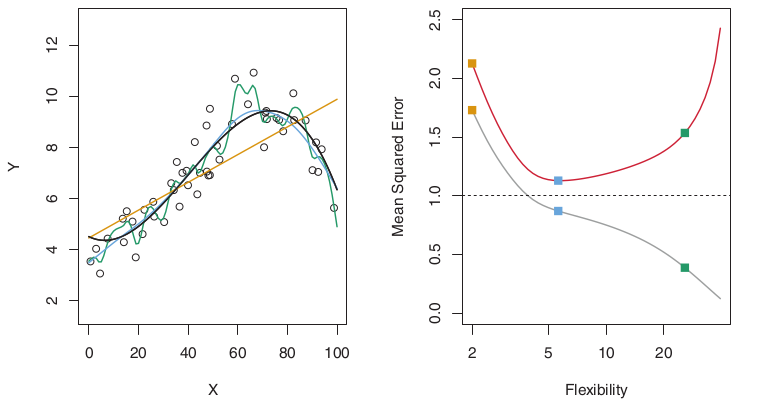
\includegraphics[width=\textwidth]{./chap/1chap/1sec/2images/2_1trainingMSEandTestMSE.png}
  \caption{Left:Data simulated from $f$, shown in black and 3 estimates
  of $f$\\Right: Training MSE in grey and test MSE in red.\\Squares
represent the training and test MSEs for the 3 fits shown in the 
left-hand pannel}
  \label{fig:2.1}
\end{figure}
The blue curve minimizes the test MSE, and visually appears to estimate
$f$ the best in the left-hand panel.\\\tR{The horizontal dashed line
indicates $\V{\epsilon}$ the irreducible error in which corresponds
to the lowest achievable test MSE among all possible methods.}\\
\tB{When a given method yields a high training MSE but a low test MSE 
we say that data are \emph{overfitting}}.

\paragraph{The Bias-Variance Trade-Off}\enc{
$\E{\left( y_{0}-\widehat{f}\left( x_{0} \right) \right)^{2}}=
\V{\widehat{f}\left( x_{0} \right)}+\left[ Bias\left( \widehat{f}
\left( x_{0} \right)\right) \right]^{2}+\V{\epsilon}$}
$\begin{cases}\E{\left(y_{0}-\widehat{f}\left(x_{0}\right)\right)^{2}}
\text{ defines the \tB{\emph{expected test MSE}} and refers to the 
average test MSE.}\\\V{\hat{f}(x_{0})}\text{ the amount by which $\widehat{f}$ 
would change if we estimating it using a different training data.}\\
\left[Bias\left(\hat{f}(x_{0})\right)\right]^{2}\text{ refers to the error that is introduced by approximating a
real-life problem.}\end{cases}$\\As we increase the flexibility of a
class methods, the bias tends to initially decrease faster than the 
variance increases. 
\begin{figure}[H]
  \centering
  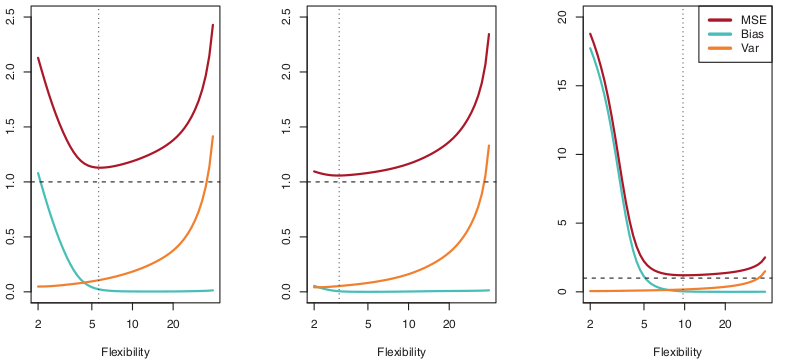
\includegraphics[width=\textwidth]{./chap/1chap/1sec/2images/2_2biaisVarianceMSE.png}
  \caption{Squared bias, variance and test MSE.\\$\V{\epsilon}$ indicates by the dashed line.}
  \label{fig:2.1}
\end{figure}
\subsection{Bias, Variance and Model Complexity}
The Loss function for measuring errors between $Y$ and $\hat{f}(X)$ is denoted by $L\left(Y,
\hat{f}(X)\right)$. Typical choices are: 
$$ L\left(Y,\hat{f}(X)\right) = 
\begin{cases}
	\left(Y-\hat{f}(X)\right)^{2}\text{ squared error}\\
	\left|Y-\hat{f(X)}\right|\text{ absolute error}
\end{cases}
$$
There are 3 important quantities:
$$ 
\begin{cases}
	\overline{err} = \dfrac{1}{N}\su{{i=1}}{N}L\left(y_{i},\hat{f}(x_{i})\right)\\
	Err_{\mathcal{T}}=\E{L\left(Y,\hat{f}(X)\right)|\mathcal{T}}\text{ \emph{Test error}}\\
	Err=\E{L\left(Y,\hat{f}(X)\right)}=\E{Err_{\mathcal{T}}}\text{ \emph{Test error}}
\end{cases}
$$
\paragraph{The classification setting}
Suppose that we seek to estimate $f$ on the basis of training 
observations $\left\{ \left( x_{i},y_{i} \right) \right\}_{1\leq i\leq
n}$ where now $\left( y_{i} \right)_{1\leq i\leq n}$ are qualitative.\\
The most common approach for quantifying the accuracy of our estimate
$\widehat{f}$ is the \tB{training \emph{error rate}}:\\
\enc{$\dfrac{1}{n}
\su{{i=1}}{n}I_{y_{i}\neq \widehat{y}_{i}}\text{ with }I_{y_{i}\neq
\widehat{y}_{i}}\begin{cases}1\Leftarrow y_{i}\neq \widehat{y}_{i}\\0
\Leftarrow y_{i}=\widehat{y}_{i}\end{cases}$}.\\ The \emph{test error
rate} associated with a set of test observation of the form $\left( 
x_{0},y_{0} \right)$ is given by:\encV{$Ave\left( I_{y_{0}\neq 
\widehat{y}_{0}} \right)$}
%\subparagraph{The Bayes Classifier}
%\sB{The test error rate is minimized, on average, by a very simply 
%classifier that assigns each observation to the most likely class}. We
%should simply assign a test observation with predictor vector $x_{0}$
%to the class $j$ for which $\ProbC{X=x_{0}}{Y=j}$ is largest.
%\begin{figure}[H]
%  \centering
%  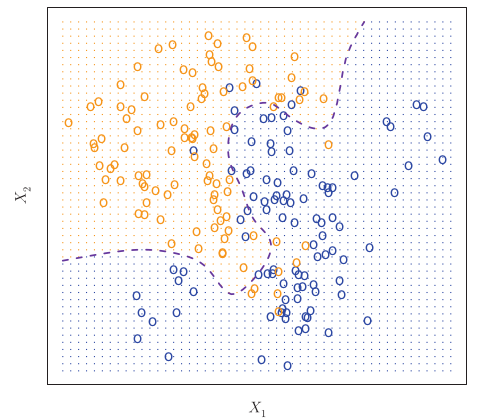
\includegraphics[width=\textwidth]{./chap/1chap/1sec/2images/2_3bayesClassifier.png}
%  \caption{A simulated data set consisting of 100 observations in each
%  of 2 groups, indicated in blue and in orange.\\The purple dashed line
%represents the \emph{Bayes decision boundary}, the orange background
%grid indicates the region in which a test observation will be assigned
%to the orange class, and likewise to blue color.}
%  \label{fig:2.2}
%\end{figure}
%The orange shaded region reflects the set of
%points for which $\ProbC{X}{Y=orange}$ is greater than $50\%$, while 
%the blue shaded region indicates the set of points for which the 
%probability is below $50\%$. The purple dashed line represents the 
%points where the probability is exactly $50\%$. \sB{Since the Bayes 
%classifier will always choose the class for which $\ProbC{X=x_{0}}{Y=j}
%$ is largest, the error rate at $X=x_{0}$ will be $1-\max\limits_{j}
%\ProbC{X=x_{0}}{Y=j}$}.\\ In general, the overall Bayes error rate is
%given by \enc{$1-\E{\max\limits_{j} \ProbC{X}{Y=j}}$}
%\subparagraph{K-Nearest neighbors}
%\sB{For real data we do not know the conditional distribution of $Y$ 
%given $X$ and so computing the Bayes classifier is impossible}.
%Therefore, the Bayes classifier serves as an unattainable gold standard
%against which to compare other methods.\\Given a positive integer $K$ 
%and a test observation $x_{0}$.
%\begin{enumerate}
%  \item It identifies the $K$ points in the training data that are
%    closet to $x_{0}$ represented by $\mathcal{N}_{0}$
%  \item It then estimates the conditional probability for class $j$ as
%    the fraction of points in $\mathcal{N}_{0}$ whose response values
%  equal $j$:$\ProbC{X=x_{0}}{Y=j}=\dfrac{1}{K}\su{{i\in\mathcal{N}_{0}}
%}{{}}I_{y_{i}=j}$
%\end{enumerate}
%\begin{figure}[H]
%  \centering
%  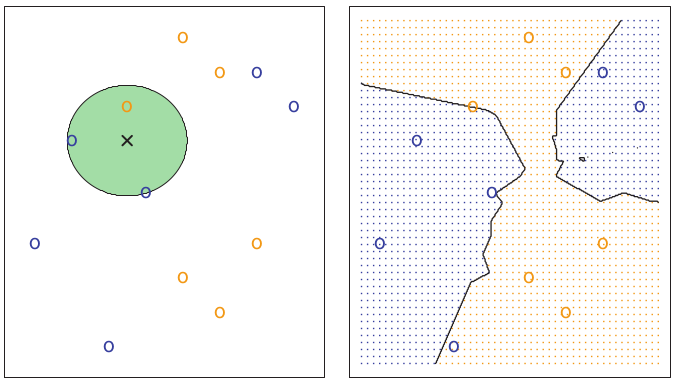
\includegraphics[width=\textwidth]{./chap/1chap/1sec/2images/2_4KNNworking.png}
%  \caption{KNN approach for $k=3$\\A test observation at which a
%  predicted class label is desired is shown as a black cross.\\
%Right-hand panel: The KNN decision boundary for this example is shown
%in black. The blue grid indicates the region in which a test 
%observation will be assigned to the blue class, likewise for the orange
%grid.}
%  \label{fig:2.2}
%\end{figure}Explanation of the KNN approach:\\
%Suppose that we choose $K=3$, then KNN will first identify the 3
%observations that are closet to the cross. This neighborhood is shown
%as a circle. It consists of 2 blue points and 1 orange point, resulting
%in estimated probabilities of $\frac{2}{3}$ for the blue class and
%$\frac{1}{3}$ for the orange class. Hence KNN will predict that the
%black cross belongs to the blue class.\\\\
%Despite the fact that is a very simple approach, KNN can often produce
%classifiers that are surprisingly close to the optimal Bayes classifier.
%\begin{figure}[H]
%  \centering
%  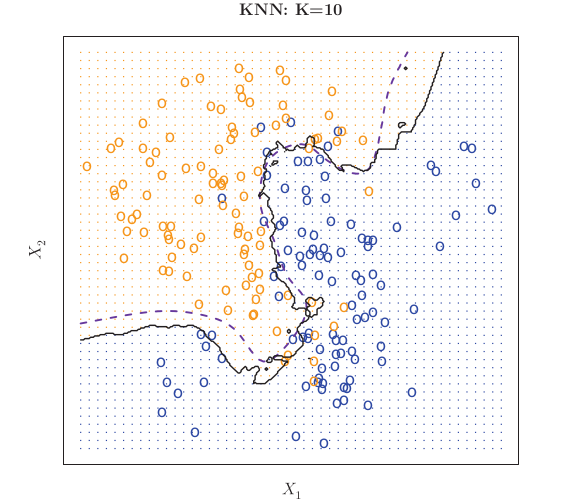
\includegraphics[width=\textwidth]{./chap/1chap/1sec/2images/2_5KNNboundary.png}
%  \caption{The black curve indicates the KNN decision boundary with
%  K=10.\\The Bayes decision boundary is shown as a purple dashed line.}
%  \label{fig:2.2}
%\end{figure}
%As $K$ grows, the method become less flexible and produces a decision
%boundary that is close to linear. This corresponds to a low-variance,
%but high-bias classifier
